\chapter{\tl{Methodology}}
\section{\tl{Data Pipeline Overview}}
\en{The data of this thesis were obtained from the Alzheimer’s Disease Neuroimaging Initiative (ADNI) database, a global research study that focuses on understanding better how to prevent or delay the disease, as well as supporting the investigation on methods of treatment. The study collects imaging, genetic, clinical, biospecimen data from people with MCI, Alzheimer’s, as well as from people that are Cognitively Normal (CN). The data was collected in 4 phases, ADNI1, ADNI2, ADNIGO and ADNI3. This study uses data from all three phases, however only uses the genetic and imaging views of the dataset. For more information on the dataset, please visit  \href{https://adni.loni.usc.edu/methods/documents/}  . \cite{69}

The imaging data is in the form of 145 ROI values, acquired from scanners either 1.5T or 3T, using T1-weighted sequences, depending on the phase. The images collected by the scanners have been filtered through Quality Control, and have been preprocessed through intensity normalization and gradient un-warping. In order to acquire the ROI intensity values, the method of MUlti-atlas region Segmentation utilizing Ensembles (MUSE) was used creating the regions of interest. ROIs values’ magnitude is analogous to the regional volume of brain tissue, depending on tissue type. The Regions that these values correspond to can be found in the appendix. (\cite{70}, \cite{71}) 

As for the genetic data, each participant has values for 54 susceptibility loci, in the form of SNPs, that have been identified by AD genetics studies. These values have been filtered through QC, and as previously mentioned are int the form of number of alleles (0,1,2) for each SNP. (\cite{72}, \cite{73}, \cite{74}, \cite{75})
\begin{figure}
  \centering
  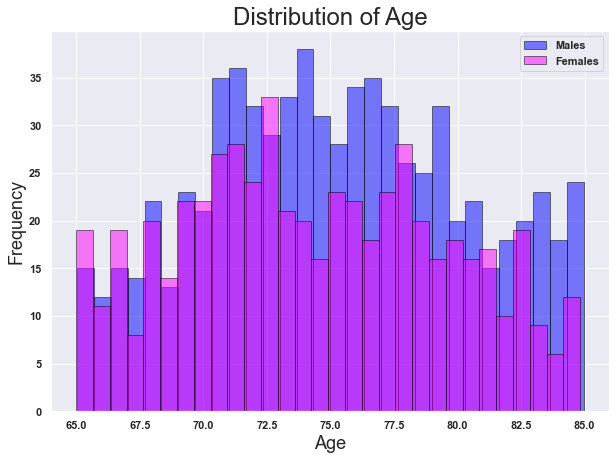
\includegraphics[width=.7\linewidth]{figures/Methodology/sex_histogram.png}
  \caption{\en{Distribution of age for participants}}
\end{figure}%
\begin{figure}
  \centering
  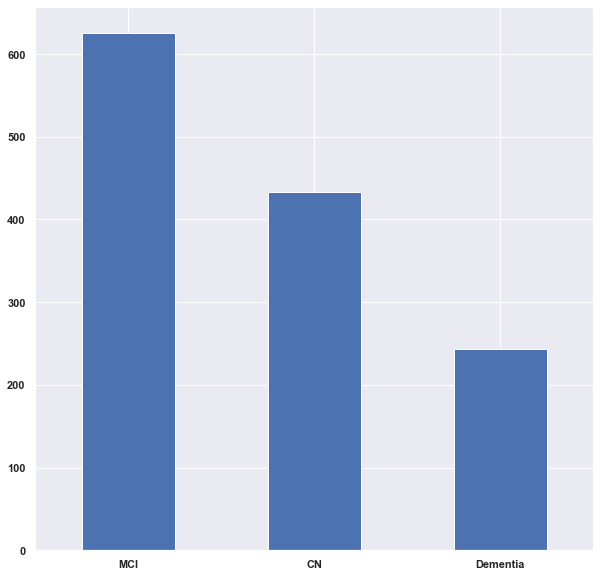
\includegraphics[width=.7\linewidth]{figures/Methodology/classes_bars.png}
  \caption{\en{Distribution of classes for participants}}
\end{figure}
\bigbreak
The dataset has 1302 participants, (56.91\% male), with mean age 75.20 y.o. for males and 74.36 y.o. for females. The dataset now has 433 CN participants (33.25\%), 626 MCI patients (48.07\%) and 243 AD patients (18.66\%). Following that, Linear Regression was performed to remove any unwanted age, sex, or brain size related effect. The regressor was fitted on the CN group, and the transformation was applied to the entire sample. Subsequently, the data was transformed through experimentation, and the output of the method was stored, in order to be compared with the raw data. Afterwards, data analysis techniques were applied, such as OPNMF to the imaging data, or MCA to the genetic data, or FAMD to the whole dataset. These methods were applied both to the original data, as well as the output of the DCCA method, in order to be compared later. The result of each one of those techniques was then saved for later tasks. Finally, each one of the results of combinations of the methods was fed to SVM as well as ensemble classifiers. 
\begin{figure}[H]
    \centering
    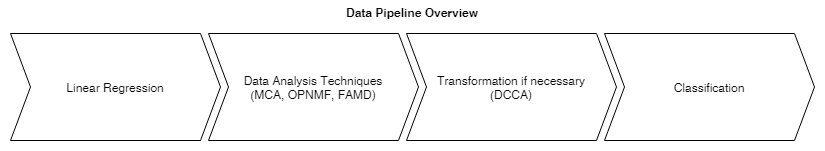
\includegraphics[width=\textwidth]{figures/Methodology/Data_Pipeline_Overview.png}
    \caption{\en{Data Pipeline Overview}}
\end{figure}
\begin{figure}[H]
    \centering
    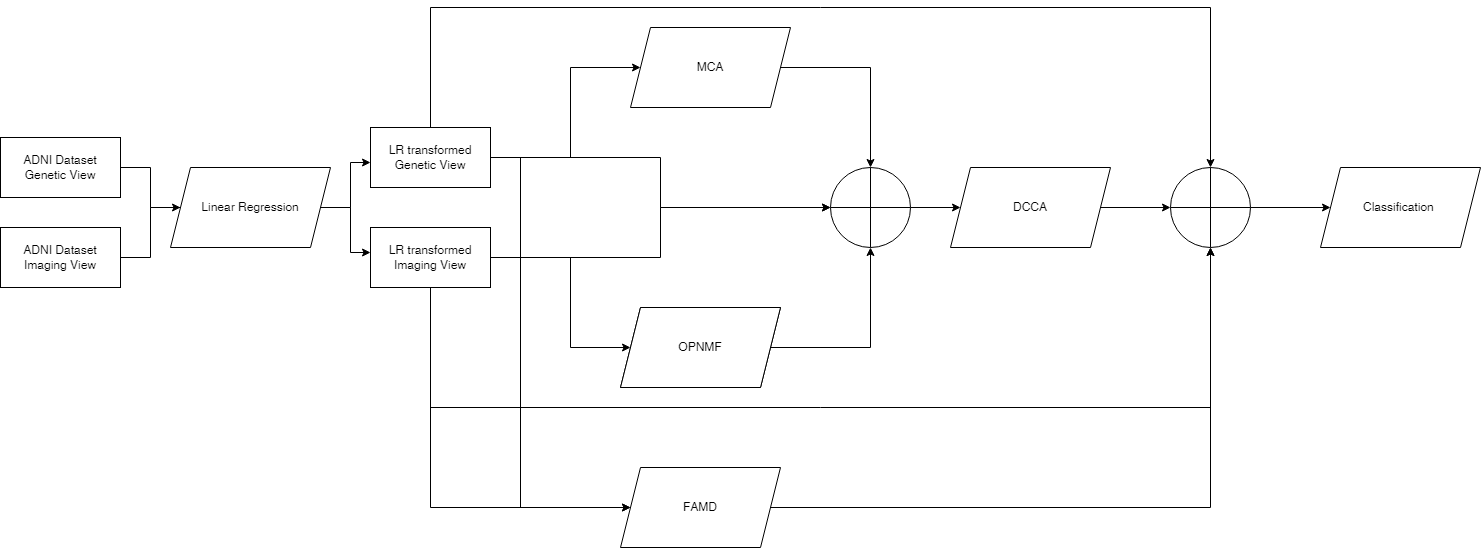
\includegraphics[width=\textwidth]{figures/Methodology/Data_Pipeline_Diagram_1.png}
    \caption{\en{Data Pipeline Diagram}}
\end{figure}
\bigbreak
}